% !TEX root = ./Basilisk-MRPROTATION-20180522.tex


\begin{figure}[htb]
	\centerline{
	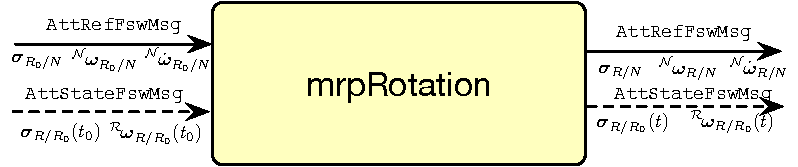
\includegraphics[]{Figures/moduleIO}
	}
	\caption{Illustration of the mrpRotation() input and output messages.  Required messages are shown with a solid line, while optional message have a dashed line.}
	\label{fig:moduleIO}
\end{figure}

\section{Model Description}
The purpose of this {\tt mrpRotation} module is to add a constant rotation relative to the input frame $\mathcal{R}_{0}$.  The output reference frame is called $\mathcal{R}$.  The initial orientation is specified through an MRP\cite{schaub} set $\bm\sigma_{R/R0}$, while the  $\mathcal{R}$-frame angular velocity vector $\leftexp{R}{\bm\omega}_{R/R0}$ is held constant in this module.  

Assume that the input reference frame $\mathcal{R}_{0}$ is given through an attitude state input message containing $\bm\sigma_{R_{0}/N}$, $\leftexp{N}{\bm\omega}_{R_{0}/N}$ and $\leftexp{N}{\dot{\bm\omega}}_{R_{0}/N}$ as illustrated in Figure~\ref{fig:moduleIO}.  The MRP set is mapped into the corresponding Direction Cosine Matrix or DCM\cite{schaub} using
\begin{equation}
	[R_{0}N] = [R_{0}N ( \bm\sigma_{R_{0}/N})]
\end{equation}


The goal of the motion is to compute the attitude of $\mathcal{R}$ relative to input frame $\mathcal{R}_{0}$ such that
\begin{align}
	\label{eq:mRot1}
	\dot{\bm\sigma}_{R/R_{0}} &= \frac{1}{4} [B(\bm\sigma_{R/R_{0}})] \leftexp{R}{\bm\omega}_{R/R_{0}}
	\\
	\label{eq:mRot2}
	\frac{\leftexp{R}{\D} {\bm\omega}_{R/R_{0}}}{\D t} &= \bm 0
\end{align}
Assume the initial $\bm\sigma_{R/R_{0}}(t_{0})$ set and the $\mathcal{R}$-frame relative invariant $\leftexp{R}{\bm\omega}_{R/R_{0}}$ vector are provided to the module.  The current $\bm\sigma_{R/R_{0}}(t_{0})$ value is then obtained by Eq.~\eqref{eq:mRot1}.  The current DCM of the $\mathcal{R}$-frame is thus
\begin{equation}
	\label{eq:mRot3}
	[RN] = [RR_{0}(\bm\sigma_{R/R_{0}}(t) ] [R_{0}N]
\end{equation}

Next, the angular velocity vector is transformed to inertial frame $\mathcal{N}$-frame components using
\begin{equation}
	\label{eq:mRot4}
	\leftexp{N}{\bm\omega}_{R/R_{0}} = [RN]^{T}\ \leftexp{R}{\bm\omega}_{R/R_{0}}
\end{equation}
to find the inertial angular velocity of the output reference frame:
\begin{equation}
	\label{eq:mRot5}
	\leftexp{N}{\bm\omega}_{R/N} = \leftexp{N}{\bm\omega}_{R/R_{0}} + \leftexp{N}{\bm\omega}_{R_{0}/N}
\end{equation}

Finally, the inertial angular acceleration of the output reference frame is found using the transport theorem:
\begin{equation}
	\label{eq:mRot6}
	\dot{\bm\omega}_{R/N} = 
	\frac{\leftexp{R}{\D} {\bm\omega}_{R/R_{0}}}{\D t} 
	 + \bm\omega_{R/N} \times {\bm\omega}_{R/R_{0}}
	+ \dot{\bm\omega}_{R_{0}/N}
	= \bm\omega_{R_{0}/N} \times {\bm\omega}_{R/R_{0}}
	+ \dot{\bm\omega}_{R_{0}/N}
\end{equation}
where $\bm\omega_{R/N} \times {\bm\omega}_{R/R_{0}} = (\bm\omega_{R/R_{0}} +\bm\omega_{R_{0}/N}) \times {\bm\omega}_{R/R_{0}} = \bm\omega_{R_{0}/N} \times {\bm\omega}_{R/R_{0}}$ is used.  Expressed in $\mathcal{N}$ frame components, this vector equation is numerically evaluated using:
\begin{equation}
	\label{eq:mRot7}
	\leftexp{N}{\dot{\bm\omega}}_{R/N} = \leftexp{N}{\bm\omega}_{R_{0}/N} \times \leftexp{N}{\bm\omega}_{R/R_{0}}
	+ \leftexp{N}{\dot{\bm\omega}}_{R_{0}/N}
\end{equation}




